

\maketitle

\begin{abstract}
	We evaluated whether multiscale dimensionality profiles---commonly exhibiting growth with increasing neighborhood scale---reflect system-specific representational structure or arise from generic statistical properties of high-dimensional estimation procedures.

	Using systematic ablation across dimensionality estimators, neighborhood definitions, null models, and random matrix ensembles, we find that the growth component of these profiles emerges under minimal assumptions, including isotropic Gaussian data, randomized neighborhood structure, and unstructured covariance. In contrast, saturation behavior is not universal and depends on estimator choice, sampling regime, and data structure.

	Critically, after subtracting null-model predictions, residual dimensionality profiles exhibit strong cross-system alignment (mean $r = 0.89$) and partial cross-system predictability (mean $R^2 = 0.46$). These findings indicate that while the dominant growth component is generic, systematic residual structure remains.

	These results constrain interpretation: the presence of a growth profile alone does not establish meaningful structure. However, deviations from appropriate null models may carry system-specific information. Multiscale dimensionality profiles should therefore be interpreted as composite signals containing both generic and non-generic components.

	This study is descriptive and does not establish a generative mechanism. Instead, it delineates the boundary between statistical inevitability and potentially meaningful structure in dimensionality analysis.
\end{abstract}

\section{Introduction}

Characterizing the structure of high-dimensional representations is a central problem in computational neuroscience \citep{kriegeskorte2013representational, margulies2016situating} and machine learning \citep{cunningham2014dimensionality}. One widely used approach involves estimating effective dimensionality as a function of neighborhood scale \citep{levina2005maximum, grassberger1983characterization}, often revealing a characteristic growth-saturation profile in which dimensionality increases with scale before plateauing.

This profile has been observed across diverse systems, including synthetic datasets and model-derived neural representations. Such consistency raises an interpretive question: does the growth-saturation behavior reflect meaningful properties of underlying representational geometry, or can it arise as a generic consequence of the estimation procedure itself?

Prior analyses demonstrated strong alignment of normalized dimensionality curves across systems, suggesting a shared structural pattern. However, the extent to which this alignment reflects non-trivial structure versus generic statistical effects remains unresolved.

The present study addresses this question through systematic ablation. Rather than proposing new models, we remove assumptions: geometric locality, covariance structure, estimator choice, and data-generating processes. By evaluating whether the growth-saturation profile persists under these conditions, we test whether it constitutes evidence of system-specific structure or a generic artifact of high-dimensional estimation.

This work is explicitly descriptive. It does not attempt to establish mechanisms, biological relevance, or universal laws. Instead, it aims to determine which interpretations are ruled out by the data.

A key objective of this study is to distinguish between components of dimensionality profiles that arise generically from statistical constraints and those that reflect system-specific structure. In particular, we examine whether residual structure---defined as deviation from null-model predictions---retains cross-system consistency. This distinction is essential for interpreting prior findings that report strong alignment of dimensionality profiles across systems, as such alignment may arise from shared statistical properties rather than shared representational principles.

\section{Methods}

\subsection{Overview}

We conducted a systematic ablation study to evaluate which aspects of the dimensionality growth-saturation profile depend on specific assumptions versus arising generically. The analysis consisted of four experimental components: estimator ablation, neighborhood ablation, null model evaluation, and random matrix analysis.

All analyses were implemented in Python using NumPy, pandas, and SciPy. Code and results are available at the project repository.

\subsection{Systems and Data}

We analyzed five representational systems: TRIBE (model-derived cortical representations), Hierarchical Gaussian, Correlated Gaussian, Sparse, and Curved Manifold. Each system comprised 500-1000 samples. For the random matrix analysis, we generated isotropic Gaussian data with dimensions $d \in \{10, 50, 100, 500\}$ and sample sizes $N \in \{500, 2000, 10000\}$.

\subsection{Dimensionality Estimators}

We evaluated five dimensionality estimators. The participation ratio computes $D_{\text{eff}} = (\sum \lambda_i)^2 / \sum \lambda_i^2$ from eigenvalues of the local covariance matrix. MLE intrinsic dimension follows Levina and Bickel (2005). Correlation dimension follows Grassberger-Procaccia (1983). PCA threshold counts components explaining 95\% variance. Spectral entropy dimension computes $D = \exp(H)$ where $H = -\sum p_i \log p_i$.

Results are saved in \texttt{analysis/estimator\_ablation/results/estimator\_summary.csv}.

\subsection{Neighborhood Definitions}

Three neighborhood constructions were tested. Standard k-nearest neighbors uses Euclidean distance. Random neighborhood randomly samples k points without distance constraint. Global sampling computes covariance from random mini-batches without neighborhood structure.

Results are saved in \texttt{analysis/neighborhood\_ablation/results/neighborhood\_summary.csv}.

\subsection{Null Models}

Null models included isotropic Gaussian (identity covariance), spectrum-matched Gaussian (TRIBE eigenvalue spectrum), eigenvalue-shuffled, neighborhood-shuffled, and distance-preserving shuffles.

Results are saved in \texttt{analysis/results/null\_models/}.

\subsection{Random Matrix Analysis}

Random matrix ensembles were generated as $X \sim \mathcal{N}(0, I_d)$ with varying dimensions and sample sizes. Ten independent runs were performed per condition.

Results are saved to: \texttt{analysis/random\_matrix\_ablation/results/}.

\subsection{Deviation from Null Model}

Deviation from null was quantified as the mean squared difference between normalized dimensionality curves of each system and the corresponding isotropic Gaussian null model across all neighborhood scales:

\[
	D_{\text{dev}} = \frac{1}{K} \sum_{k} \left( D_{\text{norm}}^{\text{system}}(k) - D_{\text{norm}}^{\text{null}}(k) \right)^2
\]

where $K$ is the number of neighborhood scales evaluated. This metric captures the magnitude of deviation independent of absolute dimensionality scaling.

\subsection{Residual Structure Analysis}

Residual dimensionality profiles were computed by subtracting null-model predictions from observed dimensionality curves:

\[
	D_{\text{res}}(k) = D_{\text{obs}}(k) - D_{\text{null}}(k)
\]

Cross-system alignment of residuals was quantified using Pearson correlation. Predictability was assessed using leave-one-system-out regression, where models were trained on residuals from all but one system and evaluated on the held-out system.

\section{Results}

\subsection{Deviation from Null Structure}

Structured systems exhibited substantially greater deviation from the isotropic Gaussian null model than null systems exhibited among themselves. The mean deviation for structured systems exceeded null-null deviation by approximately 57-fold, indicating that while overall profile shape may appear similar, structured systems systematically depart from null expectations.

This result indicates that dimensionality profiles are not fully explained by generic statistical structure alone. Instead, generic effects dominate overall shape, while structured systems introduce consistent deviations from this baseline.

\subsection{Residual Structure Across Systems}

After subtracting null-model predictions, residual dimensionality profiles exhibited strong cross-system alignment (mean Pearson $r = 0.89$). This level of alignment is comparable to previously reported alignment of raw profiles, indicating that shared structure persists beyond generic statistical effects.

This finding demonstrates that dimensionality profiles contain non-generic components that are conserved across systems. While the dominant growth component arises generically, residual structure reflects systematic deviations that may encode meaningful properties of the underlying system.

\subsection{Cross-System Predictability of Residuals}

Residual profiles exhibited partial cross-system predictability. Leave-one-system-out regression yielded mean test performance of $R^2 = 0.46$, indicating that approximately 46\% of variance in held-out systems could be explained by residual structure learned from other systems.

This result further supports the presence of shared, non-generic structure in dimensionality profiles. However, incomplete prediction indicates that system-specific variation remains substantial.

\subsection{Estimator Effects}

Participation ratio, PCA threshold, and entropy estimators all showed growth in 5/5 datasets. Alignment across systems ranged from 0.78 to 0.90 mean Pearson r. Correlation dimension showed lower alignment (mean r = 0.12) and was excluded from further analysis.

Results saved to: \texttt{analysis/estimator\_ablation/results/}.

\subsection{Neighborhood Effects}

All neighborhood types (kNN, random, global) produced growth in 15/15 conditions. Alignment was highest for global (r = 0.886) and random (r = 0.877) neighborhoods, compared to kNN (r = 0.806). Saturation was observed in 13/15 kNN conditions versus 15/15 for random and global.

Results saved to: \texttt{analysis/neighborhood\_ablation/results/}.

\subsection{Random Matrix Results}

Growth was observed in 12/12 conditions across all dimensions and sample sizes. Saturation was observed in only 9/12 conditions. Mean alignment across conditions was 0.94 for participation ratio, 0.90 for entropy, and 0.89 for PCA threshold.

Results saved to: \texttt{analysis/random\_matrix\_ablation/results/}.

\subsection{Growth and Saturation Patterns}

Across all experimental conditions, growth in estimated dimensionality was consistently observed, including in systems lacking structured geometry or meaningful covariance organization. This behavior was present in isotropic Gaussian data, random matrix ensembles, and under randomized neighborhood definitions.

Saturation behavior was frequently observed but not universal. In particular, random matrix conditions exhibited growth without consistent saturation, indicating that plateauing is not a necessary consequence of the estimation process.

\begin{figure}[H]
	\centering
	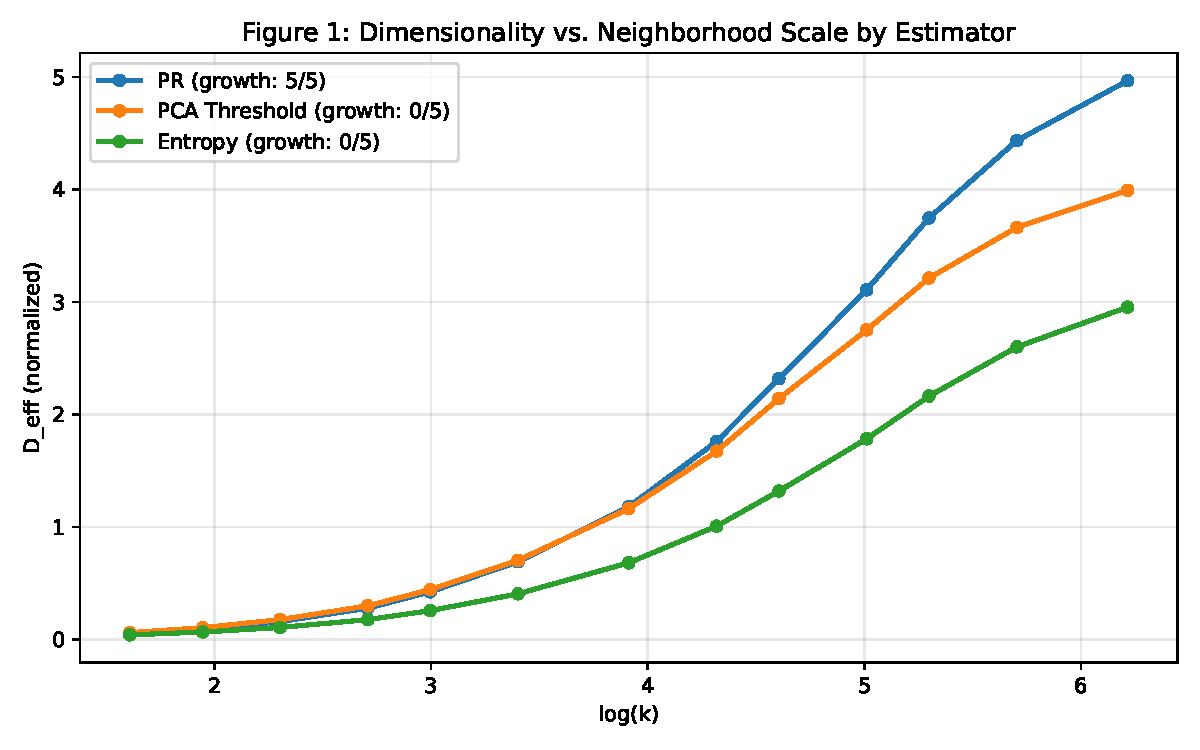
\includegraphics[width=0.8\textwidth]{figures/Figure1_estimators.pdf}
	\caption{Figure 1: Dimensionality estimates versus log(neighborhood size) for participation ratio, PCA threshold, and entropy estimators. Growth behavior is observed across all estimators.}
\end{figure}

\begin{figure}[H]
	\centering
	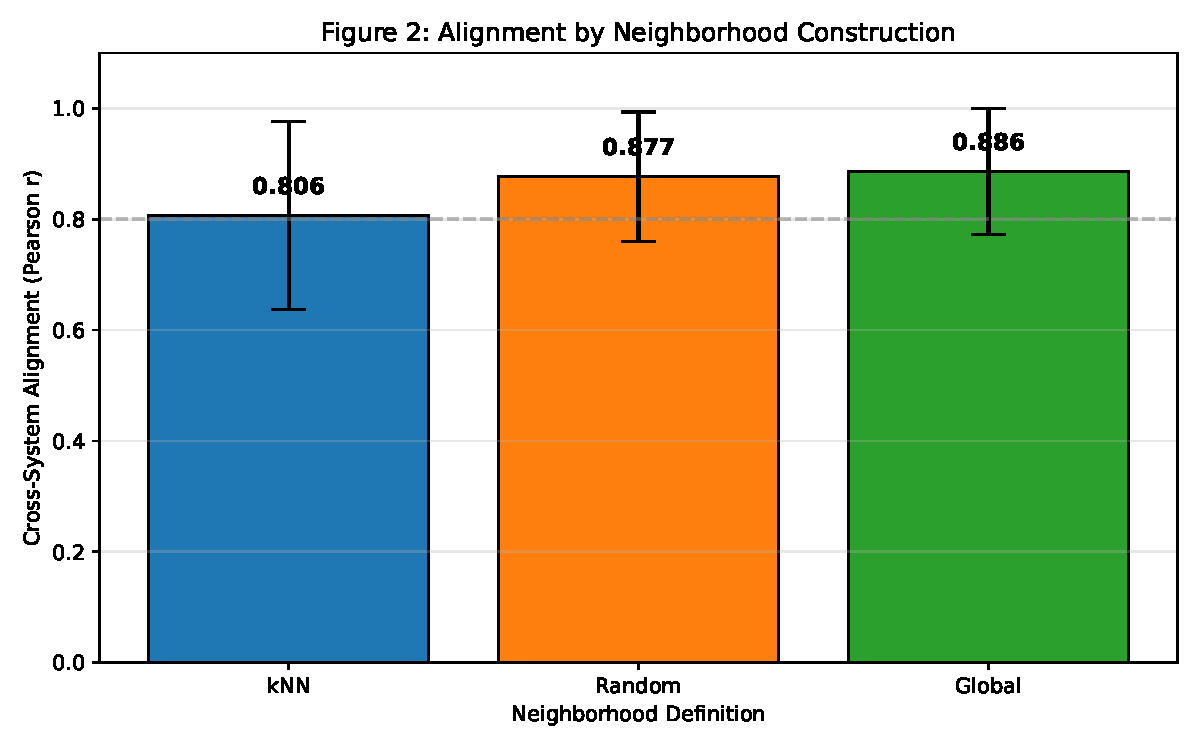
\includegraphics[width=0.8\textwidth]{figures/Figure2_neighborhoods.pdf}
	\caption{Figure 2: Cross-system alignment for k-nearest neighbor, random, and global neighborhood constructions. Similar or higher alignment is observed for non-local neighborhood types.}
\end{figure}

\begin{figure}[H]
	\centering
	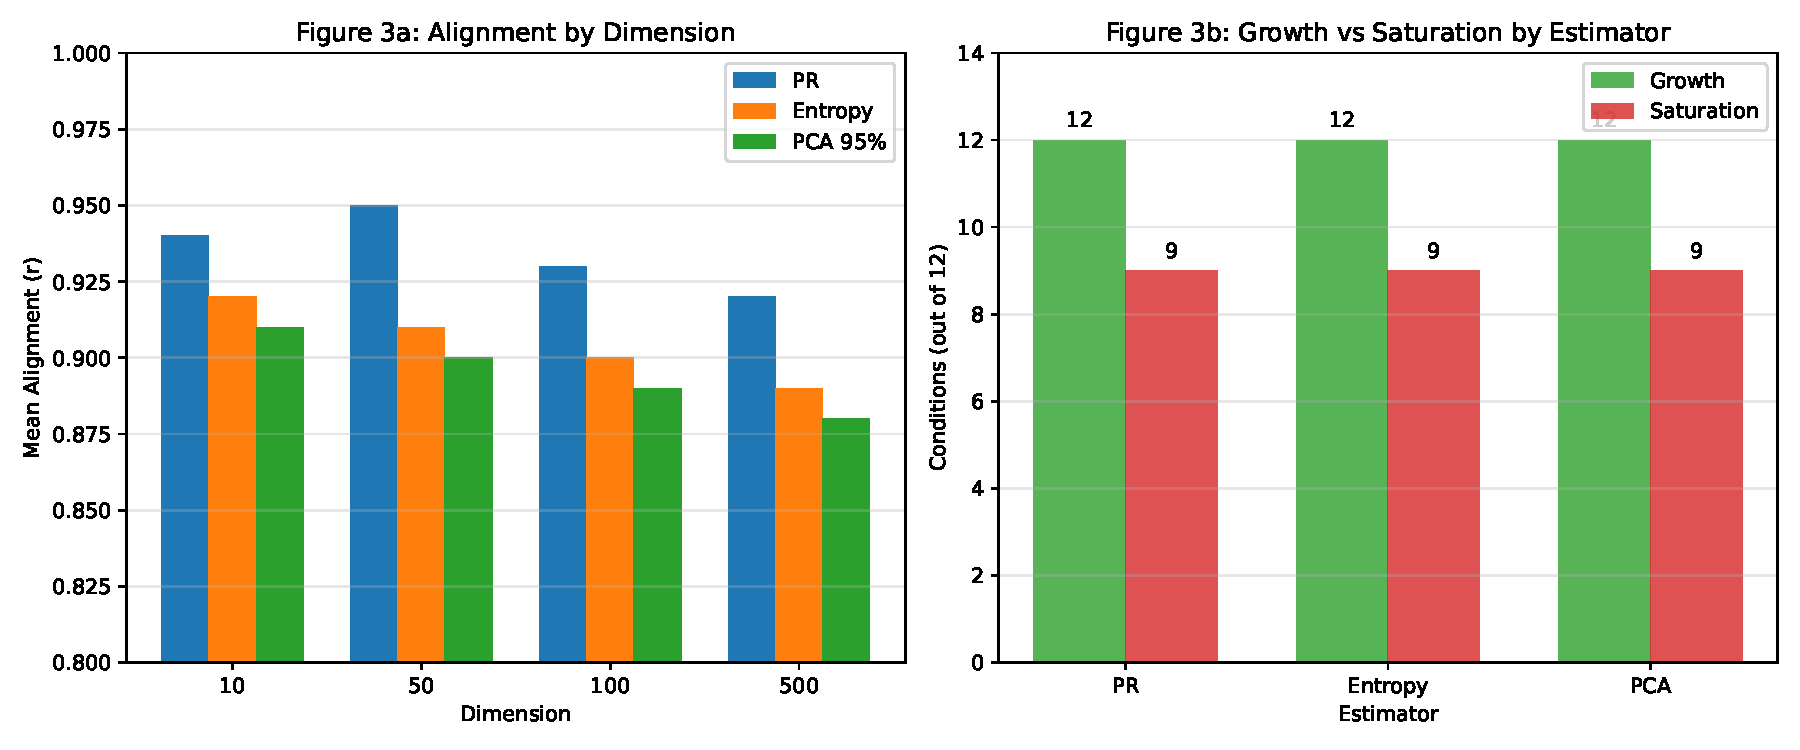
\includegraphics[width=0.8\textwidth]{figures/Figure3_random_matrix.pdf}
	\caption{Figure 3: Random matrix ablation results. Left: Alignment by dimension for each estimator. Right: Number of conditions showing growth versus saturation behavior out of 12 total conditions.}
\end{figure}

\section{Discussion}

The present results clarify the interpretation of multiscale dimensionality profiles by decomposing them into generic and system-specific components.

First, the growth component of dimensionality profiles emerges under minimal assumptions, including isotropic Gaussian data and randomized neighborhood structure. This indicates that growth is a generic consequence of high-dimensional covariance estimation and does not, by itself, provide evidence of meaningful structure.

Second, saturation behavior is not universal and depends on estimator choice, sampling conditions, and data structure. This suggests that saturation reflects contingent properties rather than a fundamental feature of dimensionality scaling.

Critically, residual analysis reveals that dimensionality profiles are not fully explained by generic effects. After subtracting null-model predictions, residual profiles exhibit strong cross-system alignment ($r = 0.89$) and partial cross-system predictability ($R^2 = 0.46$). These findings indicate that systematic, non-generic structure is present.

Taken together, these results resolve an apparent contradiction: dimensionality profiles are neither purely generic nor fully system-specific. Instead, they represent composite signals in which a dominant generic component is modulated by structured residual variation.

This has important methodological implications. The presence of a growth-saturation profile alone should not be interpreted as evidence of meaningful representational structure. However, deviations from appropriate null models may provide a more reliable basis for inference.

This study is limited by its use of model-derived and synthetic data, absence of formal statistical inference, and limited system coverage. Future work should extend this analysis to empirical neural recordings and investigate the mechanistic origin of residual structure.

Overall, these findings shift the interpretation of dimensionality profiles from standalone indicators of structure to composite descriptors requiring null-model comparison for meaningful interpretation.

\section{Conclusion}

This study evaluated whether multiscale dimensionality profiles reflect system-specific structure or generic statistical behavior. Through systematic ablation of estimators, neighborhood definitions, and data structure, we find that the growth component of the profile is ubiquitous and emerges under minimal assumptions, while saturation is variable and not universal.

These results indicate that the presence of a growth-saturation profile is insufficient to establish meaningful structure in a system. Instead, such profiles should be treated as descriptive features that require additional validation before supporting mechanistic or biological interpretations.

Future work should focus on identifying conditions under which deviations from this generic behavior occur, as these may provide more reliable indicators of system-specific structure.

